\newpage

\section{Appendice C: La Règle de la Chaîne}

\begin{definitionbox}[Règle de la Chaîne]
La \textbf{règle de la chaîne} permet de calculer la dérivée d'une fonction composée. Si $y = f(u)$ et $u = g(x)$, alors la fonction composée $y = f(g(x))$ a pour dérivée :
$$ \frac{dy}{dx} = \frac{dy}{du} \cdot \frac{du}{dx} = f'(g(x)) \cdot g'(x) $$
Cette règle exprime que la variation de $y$ par rapport à $x$ est le produit des variations intermédiaires.
\end{definitionbox}

\subsection{Construction pas à pas de la règle de la chaîne}

\begin{intuitionbox}[De la dérivée simple à la composition]
L'objectif fondamental de la règle de la chaîne est de gérer les fonctions imbriquées. Au lieu de dériver directement une expression complexe, on la \textbf{décompose en couches} et on dérive chaque couche successivement. Le principe clé : \textbf{on dérive de l'extérieur vers l'intérieur}, en multipliant les dérivées à chaque étape.

Prenons l'exemple du calcul de la dérivée de $y = \sin(x^2)$.

\begin{enumerate}
    \item \textbf{Identification : Reconnaître la composition}
    \newline
    \textbf{Objectif :} Identifier les fonctions emboîtées pour appliquer la règle.
    \newline
    \textbf{Notre cas :} $y = \sin(x^2)$ est une composition de deux fonctions :
    \begin{itemize}
        \item Fonction extérieure : $f(u) = \sin(u)$
        \item Fonction intérieure : $u = g(x) = x^2$
    \end{itemize}
    \textbf{Notation :} On peut écrire $y = f(g(x))$ ou $y = (f \circ g)(x)$.

    \item \textbf{Première dérivation : La couche extérieure}
    \newline
    \textbf{Objectif :} Dériver la fonction extérieure par rapport à son argument, sans toucher à l'intérieur.
    \newline
    \textbf{Calcul :} On dérive $\sin(u)$ par rapport à $u$ :
    $$ \frac{dy}{du} = \cos(u) = \cos(x^2) $$
    \textbf{Interprétation :} On garde $x^2$ intact à l'intérieur du cosinus. Cette dérivée partielle nous dit comment $y$ change quand $u$ change.

    \item \textbf{Seconde dérivation : La couche intérieure}
    \newline
    \textbf{Objectif :} Dériver la fonction intérieure par rapport à la variable originale $x$.
    \newline
    \textbf{Calcul :}
    $$ \frac{du}{dx} = \frac{d}{dx}(x^2) = 2x $$
    \textbf{Interprétation :} Cette dérivée nous dit comment $u$ change quand $x$ change.

    \item \textbf{Multiplication finale : Combiner les dérivées}
    \newline
    \textbf{Objectif :} Appliquer la règle de la chaîne en multipliant les deux dérivées.
    \newline
    \textbf{Calcul :}
    $$ \frac{dy}{dx} = \frac{dy}{du} \cdot \frac{du}{dx} = \cos(x^2) \cdot 2x = 2x\cos(x^2) $$
    \textbf{Résultat final :} La dérivée de $\sin(x^2)$ est $\mathbf{2x\cos(x^2)}$.

    \item \textbf{Notation alternative : Leibniz}
    \newline
    La notation de Leibniz rend la règle intuitive : les "$du$" se "simplifient" symboliquement :
    $ \frac{dy}{dx} = \frac{dy}{du} \cdot \frac{du}{dx} $
    Bien que ce ne soit pas une vraie simplification algébrique, cette visualisation aide à retenir la structure de la règle.

    \item \textbf{Compositions multiples : Chaînes plus longues}
    \newline
    Pour trois fonctions ou plus, on continue à multiplier les dérivées.
    \newline
    \textbf{Exemple :} Si $y = f(g(h(x)))$, alors :
    $$ \frac{dy}{dx} = f'(g(h(x))) \cdot g'(h(x)) \cdot h'(x) $$
    \textbf{Cas concret :} Pour $y = e^{\sin(x^2)}$ :
    \begin{align*}
    \frac{dy}{dx} &= e^{\sin(x^2)} \cdot \frac{d}{dx}[\sin(x^2)] \\
    &= e^{\sin(x^2)} \cdot \cos(x^2) \cdot 2x \\
    &= 2x \cos(x^2) e^{\sin(x^2)}
    \end{align*}
\end{enumerate}
\end{intuitionbox}

\subsection{Intuition géométrique de la règle de la chaîne}

\begin{intuitionbox}[Interpréter la règle comme un taux de changement composé]
Une dérivée simple $f'(x)$ mesure le taux de changement instantané de $f$ par rapport à $x$. La règle de la chaîne mesure le \textbf{taux de changement à travers une variable intermédiaire}.

\textbf{Analogie physique : Vitesse et position}
\newline
Supposons qu'une particule se déplace sur un axe et que sa position $s$ dépend du temps $t$ selon $s = t^3$. Sa température $T$ dépend de sa position selon $T = \sqrt{s}$. Quelle est la variation de température par rapport au temps ?

La règle de la chaîne nous dit :
$$ \frac{dT}{dt} = \frac{dT}{ds} \cdot \frac{ds}{dt} = \frac{1}{2\sqrt{s}} \cdot 3t^2 = \frac{3t^2}{2\sqrt{t^3}} = \frac{3t^2}{2t^{3/2}} = \frac{3\sqrt{t}}{2} $$

La variation de $T$ par rapport à $t$ est le produit :
\begin{itemize}
    \item de la sensibilité de $T$ aux changements de position ($\frac{dT}{ds}$)
    \item et de la vitesse de changement de position ($\frac{ds}{dt}$)
\end{itemize}

\textbf{Cas particulier : Amplification ou atténuation}
\newline
Si $|g'(x)| > 1$, la fonction intérieure "amplifie" les variations de $x$.
\newline
Si $|g'(x)| < 1$, elle les "atténue".
\newline
La règle de la chaîne capture cet effet multiplicatif.

\tcblower
\centering
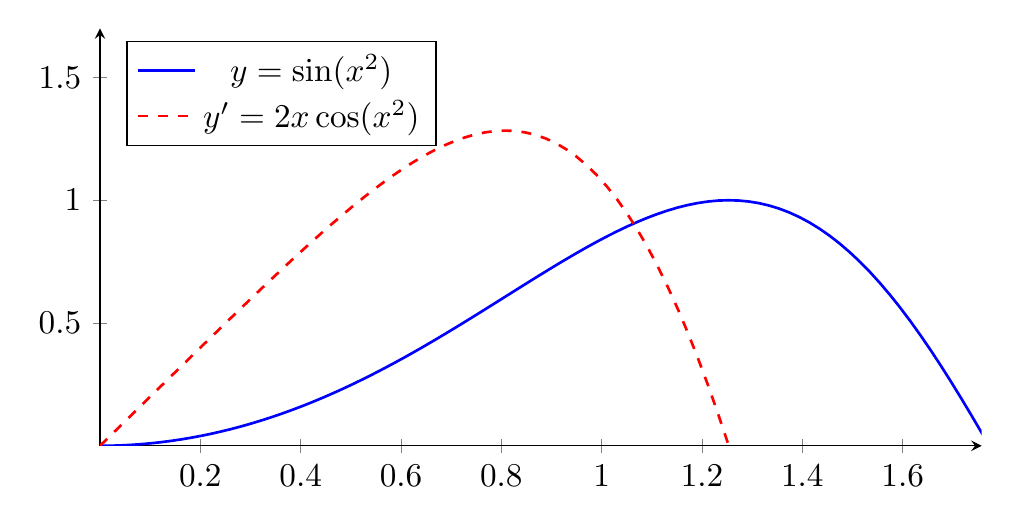
\begin{tikzpicture}[scale=1.2]
    \begin{axis}[
        axis lines=middle,
        domain=0:2,
        samples=100,
        height=6cm,
        width=0.9\linewidth,
        ymin=0, ymax=1.7,
        legend pos=north west,
    ]
    
    \addplot[blue, thick] {sin(deg(x^2))};
    \addlegendentry{$y=\sin(x^2)$}
    
    \addplot[red, dashed, thick] {2*x*cos(deg(x^2))};
    \addlegendentry{$y'=2x\cos(x^2)$}
    
    \end{axis}
\end{tikzpicture}
\par\small\textit{La fonction $\sin(x^2)$ et sa dérivée obtenue par la règle de la chaîne. La pente s'annule quand $\cos(x^2)=0$ ou $x=0$.}
\end{intuitionbox}


\subsection{Applications classiques de la règle de la chaîne}

\begin{theorembox}[Formules dérivées courantes avec composition]
Voici les applications les plus fréquentes de la règle de la chaîne :
\begin{align*}
\frac{d}{dx}[f(x)^n] &= n \cdot f(x)^{n-1} \cdot f'(x) \quad \text{(règle de puissance généralisée)} \\
\frac{d}{dx}[e^{f(x)}] &= e^{f(x)} \cdot f'(x) \\
\frac{d}{dx}[\ln(f(x))] &= \frac{f'(x)}{f(x)} \\
\frac{d}{dx}[\sin(f(x))] &= \cos(f(x)) \cdot f'(x) \\
\frac{d}{dx}[\cos(f(x))] &= -\sin(f(x)) \cdot f'(x)
\end{align*}
\end{theorembox}

\begin{intuitionbox}[Stratégie pour des compositions complexes]
Face à une fonction compliquée, une approche systématique évite les erreurs.

\textbf{Exemple : $\displaystyle y = \ln\left(\frac{1+\sqrt{x}}{1-\sqrt{x}}\right)$}

\textbf{Stratégie 1 : Décomposition explicite}
\newline
Posons des variables intermédiaires :
\begin{align*}
u &= \sqrt{x} = x^{1/2}, \quad \frac{du}{dx} = \frac{1}{2\sqrt{x}} \\
v &= \frac{1+u}{1-u}, \quad \frac{dv}{du} = \frac{(1-u) - (1+u)(-1)}{(1-u)^2} = \frac{2}{(1-u)^2} \\
y &= \ln(v), \quad \frac{dy}{dv} = \frac{1}{v}
\end{align*}

Application de la règle de la chaîne :
$$ \frac{dy}{dx} = \frac{dy}{dv} \cdot \frac{dv}{du} \cdot \frac{du}{dx} = \frac{1}{v} \cdot \frac{2}{(1-u)^2} \cdot \frac{1}{2\sqrt{x}} $$

Substitution :
$$ = \frac{1}{\frac{1+\sqrt{x}}{1-\sqrt{x}}} \cdot \frac{2}{(1-\sqrt{x})^2} \cdot \frac{1}{2\sqrt{x}} = \frac{1-\sqrt{x}}{1+\sqrt{x}} \cdot \frac{2}{(1-\sqrt{x})^2} \cdot \frac{1}{2\sqrt{x}} $$

Simplification :
$$ = \frac{1}{(1+\sqrt{x})(1-\sqrt{x})} \cdot \frac{1}{\sqrt{x}} = \frac{1}{(1-x)\sqrt{x}} $$

\textbf{Stratégie 2 : Simplification avant dérivation}
\newline
On peut parfois simplifier avec les propriétés des logarithmes :
$$ y = \ln(1+\sqrt{x}) - \ln(1-\sqrt{x}) $$

Puis dériver directement :
$$ \frac{dy}{dx} = \frac{1}{1+\sqrt{x}} \cdot \frac{1}{2\sqrt{x}} - \frac{1}{1-\sqrt{x}} \cdot \frac{-1}{2\sqrt{x}} = \frac{1}{2\sqrt{x}} \left(\frac{1}{1+\sqrt{x}} + \frac{1}{1-\sqrt{x}}\right) $$

Réduction au même dénominateur :
$$ = \frac{1}{2\sqrt{x}} \cdot \frac{2}{1-x} = \frac{1}{(1-x)\sqrt{x}} $$

\textbf{Leçon :} Toujours chercher à simplifier l'expression avant de dériver. Les propriétés algébriques peuvent considérablement réduire la complexité du calcul.

\end{intuitionbox}